\section{Leyes de maxwell}\index{Leyes de maxwell}
Se presentan las ecuaciones de Maxwell en la tabla \ref{tab:maxwell}.
\begin{table}[]
\begin{tabular}{|l|l|l|}
\hline
\rowcolor[HTML]{0066cc} 
Forma diferencial & Forma integral                                                                 & Comentario\\ \hline
$\nabla\cdot \textbf{D}=\rho_v$  & $\oint_S\textbf{D}\cdot d\textbf{S}=\int_v\rho_vdv                                 $ & Ley de Gauss\\ \hline
$\nabla\cdot \textbf{B}=0$ & $\oint_S\textbf{B}\cdot d\textbf{S}=0
$ & No existencia de monopolos \\ \hline
$\nabla\times \textbf{E}=-\frac{\partial \textbf{B}}{\partial t}$    & $\oint_L\textbf{E}\cdot dl=-\frac{\partial}{\partial t}\int_S\textbf{B}\cdot dS
$ & Ley de Faraday\\ \hline
$\nabla\times \textbf{H}=\textbf{J} + \frac{\partial \textbf{D}}{\partial t}$ & $\oint_L\textbf{H}\cdot dl=\int_S\left(\textbf{J} + \frac{\partial \textbf{D}}{\partial t}\right)\cdot d\textbf{S}$ & Ley de circuitos de Ampere \\ \hline
\end{tabular}
\caption{Leyes de Maxwell}
\label{tab:maxwell}
\end{table}
Donde es necesario recordar el operador DEL (\ref{subsec:DEL})
\begin{itemize}
\item El gradiente de un escalar V: $\nabla$V
\item La divergencia de un vector A: $\nabla\cdot$A
\item La rotacional de un vector A: $\nabla\times$A
\item El Laplaciano de un escalar V: $\nabla^2$V
\end{itemize}
Además se tienen ecuaciones auxiliares:
\begin{subequations}
\begin{align}
\intertext{Relación entre la Densidad de Campo Eléctrico y la Intensidad de Campo Eléctrico.}
\textbf{D}&= \epsilon \textbf{E}\\
\intertext{Relación entre la Densidad de Campo Magnético y la Intensidad de Campo Magnético.}
\textbf{B}&=u\textbf{H}\\
\intertext{Densidad de Corriente de conducción.}
\textbf{J}&=\sigma\textbf{E}\\
\intertext{Densidad de Corriente de convección en función de la densidad de carga volumétrica.}
\textbf{J}&=\rho_v\textbf{v}
\end{align}
\end{subequations}
Hay ligeras modificaciones si son para conductores malos (aislantes):
\begin{subequations}
\begin{align}
\textbf{D}&= \epsilon \textbf{E} + P\\
\textbf{B}&=u(\textbf{H} + M)
\end{align}
\end{subequations}
Donde P es el campo de polarización y M es el campo de magnetización, cuando el dieléctrico es lineal se tiene:
\begin{align*}
&P=\chi_e\epsilon_0\textbf{E} &M=\chi_m\textbf{H}
\end{align*}
\begin{figure}[H]
\centering
\subfloat[Ecuación de onda para campos eléctricos.]{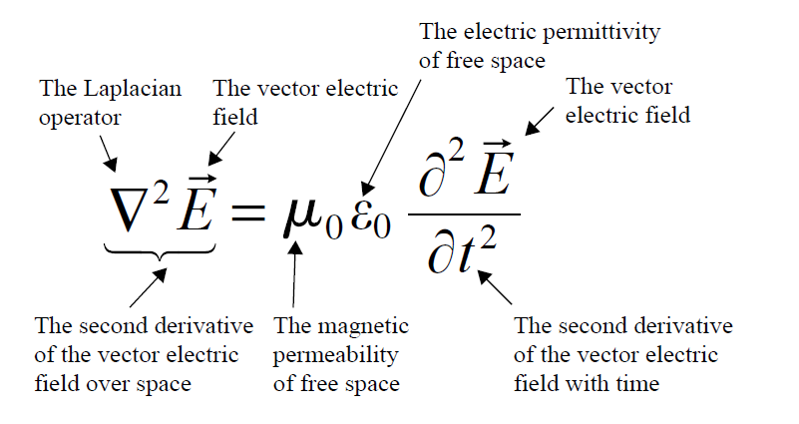
\includegraphics[width=0.8\linewidth]{LT/LT1.png}}\\
\subfloat[Ecuación de onda para campos magnéticos.]{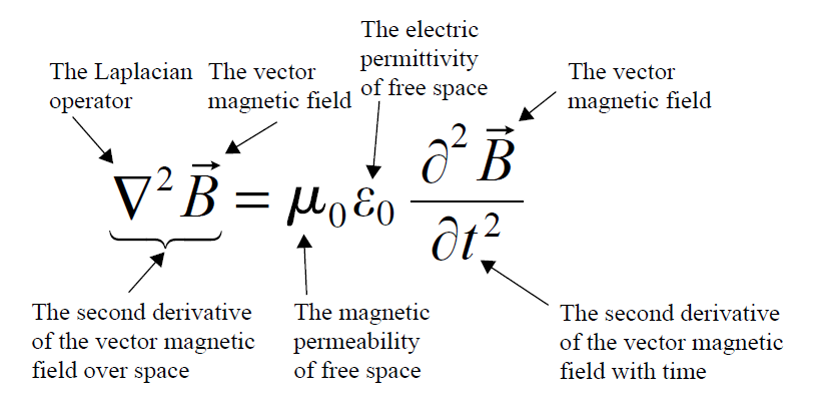
\includegraphics[width=0.8\linewidth]{LT/LT2.png}}
\caption{Ecuaciones de onda}
\end{figure}
%\section{Modelo electromagnético y las leyes de Maxwell}
